\documentclass[12pt]{article}

\usepackage[a4paper]{geometry}
\usepackage{graphicx}
\usepackage[position=b]{subcaption}
\captionsetup[subfigure]{width=0.9\textwidth}

\usepackage{booktabs} % For professional looking tables
\usepackage{multirow}

\usepackage{amsfonts}
\usepackage{amsmath}
\usepackage{amssymb}
\usepackage[T1]{fontenc}
\usepackage{siunitx} % use this package module for SI units

\usepackage{lineno}
\linenumbers

\usepackage{xspace}
\newcommand\geant{\textsc{Geant\,4}\xspace}
\newcommand\mokka{\textsc{Mokka}\xspace}
\newcommand\ddhep{\textsc{DD4hep}\xspace}
\newcommand\ilcsoft{\textsc{ILCSoft}\xspace}
\newcommand\cpp{\textsc{C++}\xspace}
\newcommand\marlin{\textsc{Marlin}\xspace}
\newcommand\lcio{\textsc{LCIO}\xspace}
\newcommand\qt{\textsc{Qt}\xspace}

\usepackage{epstopdf}

\begin{document}

\section{Additional Plots First Draft}

\begin{figure}[htbp!]
  \begin{subfigure}[t]{0.49\textwidth}
    \centering
    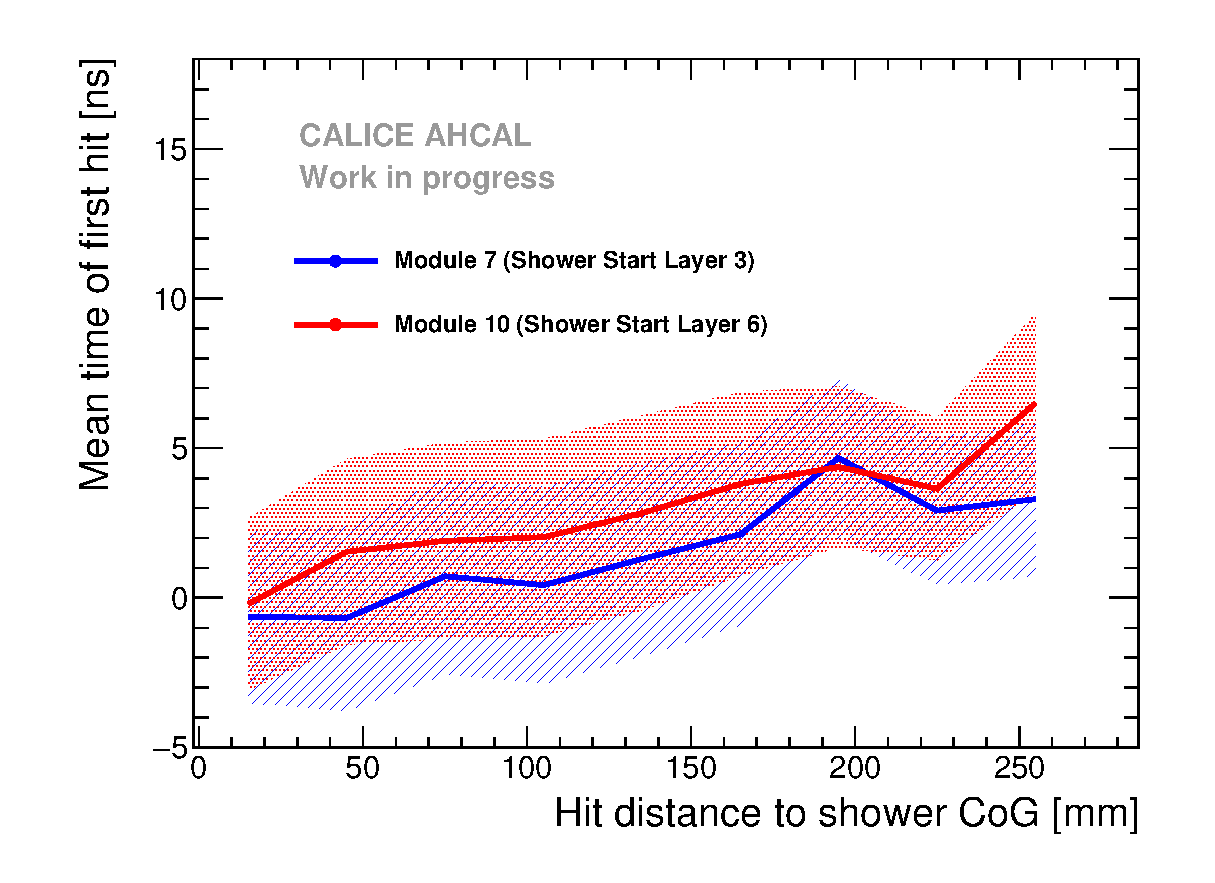
\includegraphics[width=1\textwidth]{../../Draft/fig/Timing_Radius_Comparison_ShortAsymRange_ShowerStart.eps}
    \caption{}\label{fig:Radius_FHI}
  \end{subfigure}
  \hfill
  \begin{subfigure}[t]{0.49\textwidth}
    \centering
    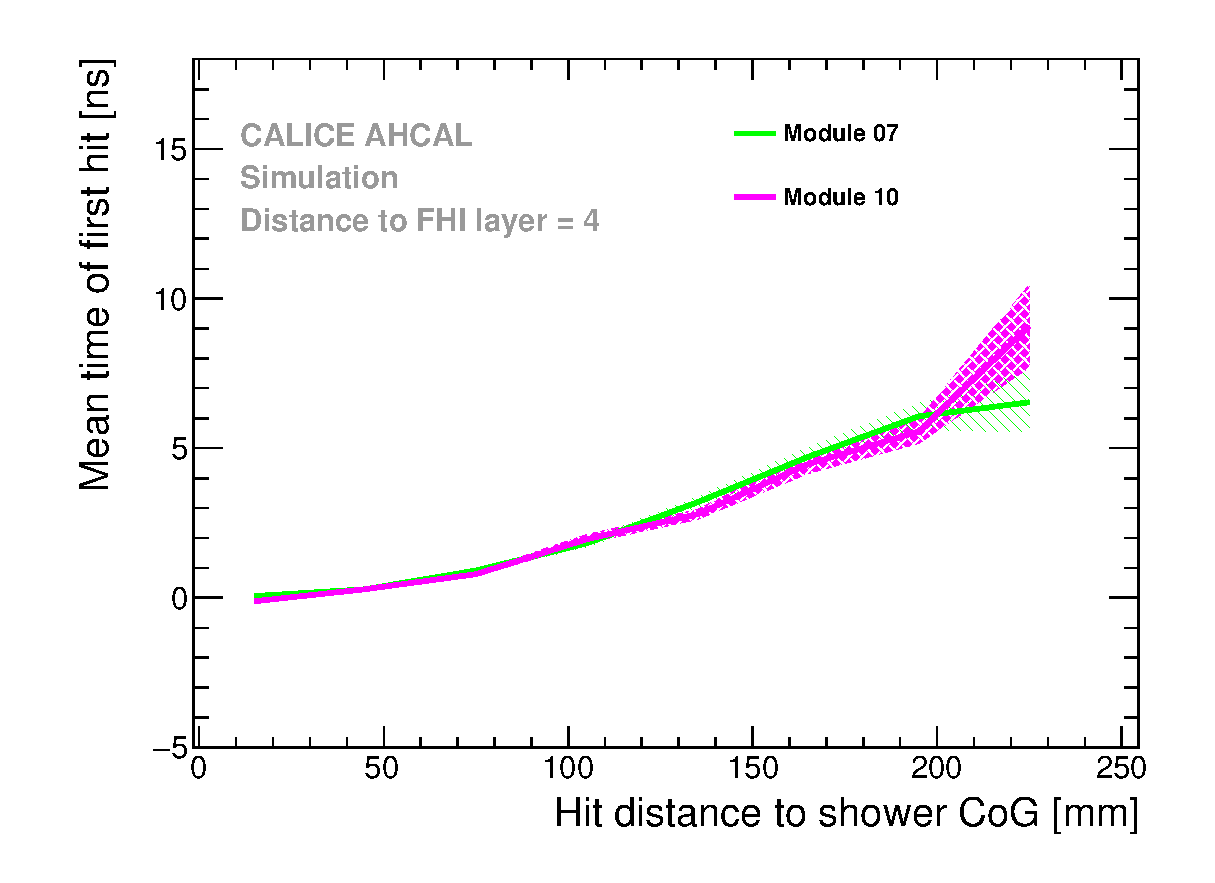
\includegraphics[width=1\textwidth]{../../Draft/fig/Radius_ShowerStartTruth.eps}
    \caption{}\label{fig:Radius_FHISim1}
  \end{subfigure}
  \caption{Mean time of first hit as a function of the hit distance to the shower axis for 50 GeV pions for a fixed distance of 4 between the reconstructed FHI layer and a layer. The left plot shows the radial timing profile of modules 7 and 10 in data. The right plots shows the radial timing profile for the same layers in simulation with the QGSP\_BERT\_HP physics list.}
  \label{fig:Radius_FHIAll}
\end{figure}

\begin{figure}[htbp!]
  \begin{subfigure}[t]{0.49\textwidth}
    \centering
    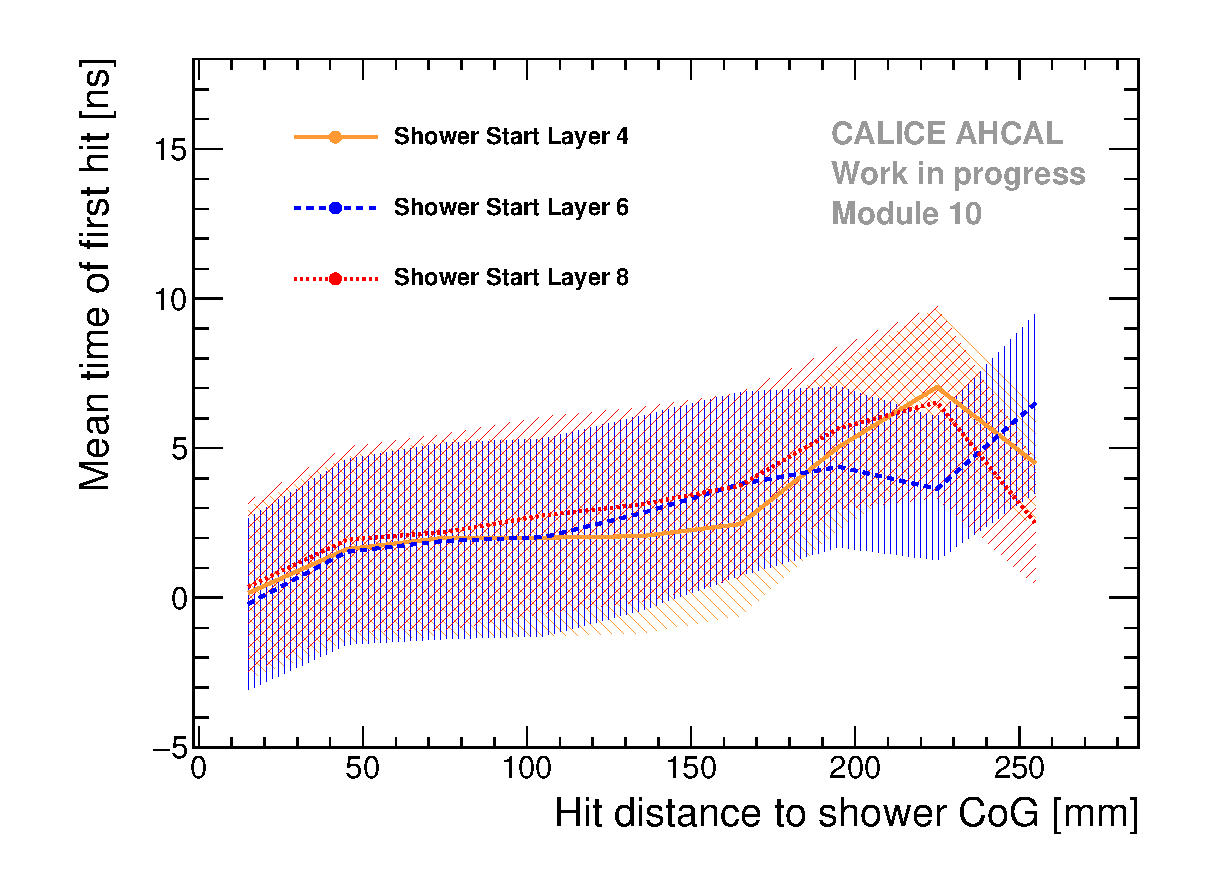
\includegraphics[width=1\textwidth]{../../Draft/fig/Timing_Radius_Comparison_ShortAsymRange_ShowerStart_FixedModule.eps}
    \caption{}\label{fig:Radius_FHI_Fixed}
  \end{subfigure}
  \hfill
  \begin{subfigure}[t]{0.49\textwidth}
    \centering
    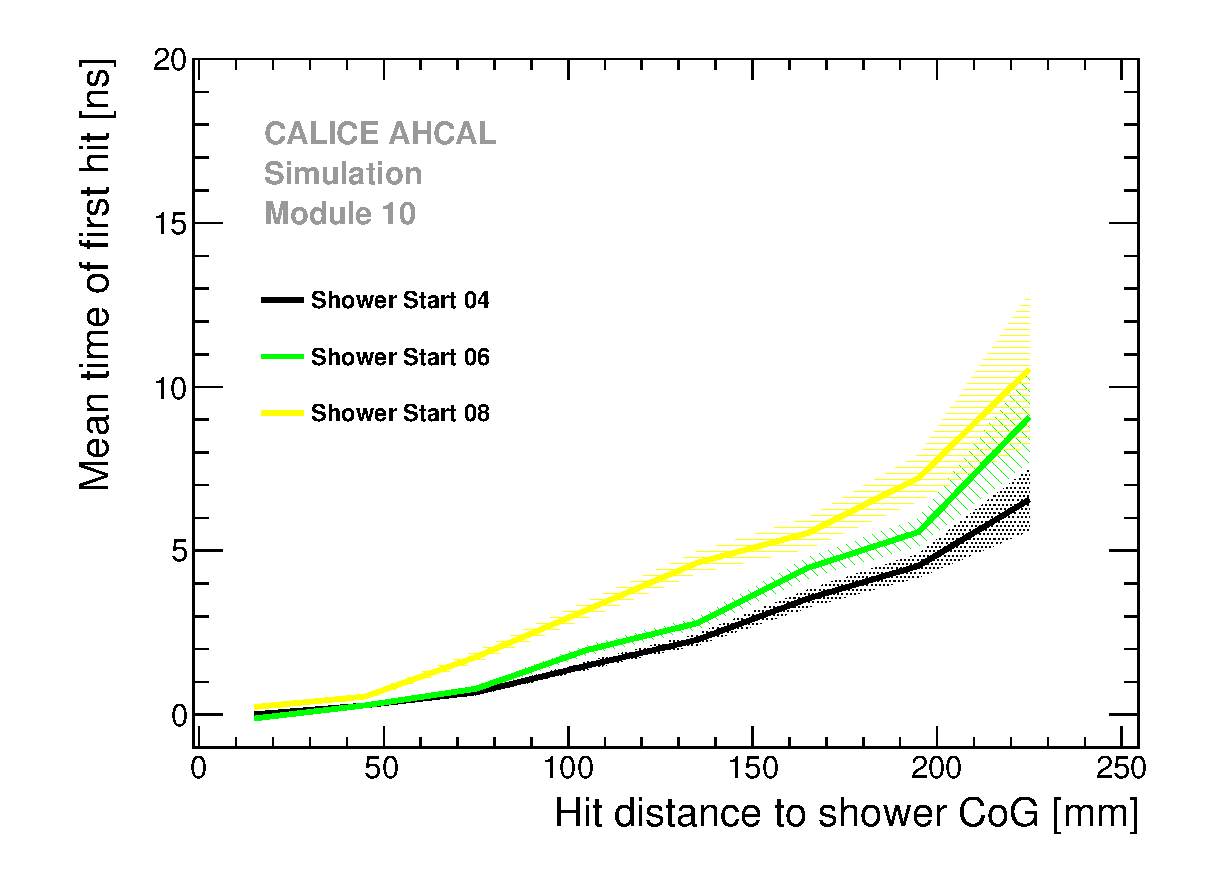
\includegraphics[width=1\textwidth]{../../Draft/fig/Radius_ShowerStartTruth_FixedModule.eps}
    \caption{}\label{fig:Radius_FHI_FixedSim}
  \end{subfigure}
  \caption{Mean time of the first hit as a function of the hit distance to the shower axis for 50 GeV pions for different reconstructed FHI layers. In data on the left and in simulation with the QGSP\_BERT\_HP physics list on the right.}
  \label{fig:Radius_FHISim}
\end{figure}

\begin{figure}[htbp!]
  \begin{subfigure}[t]{0.49\textwidth}
    \centering
    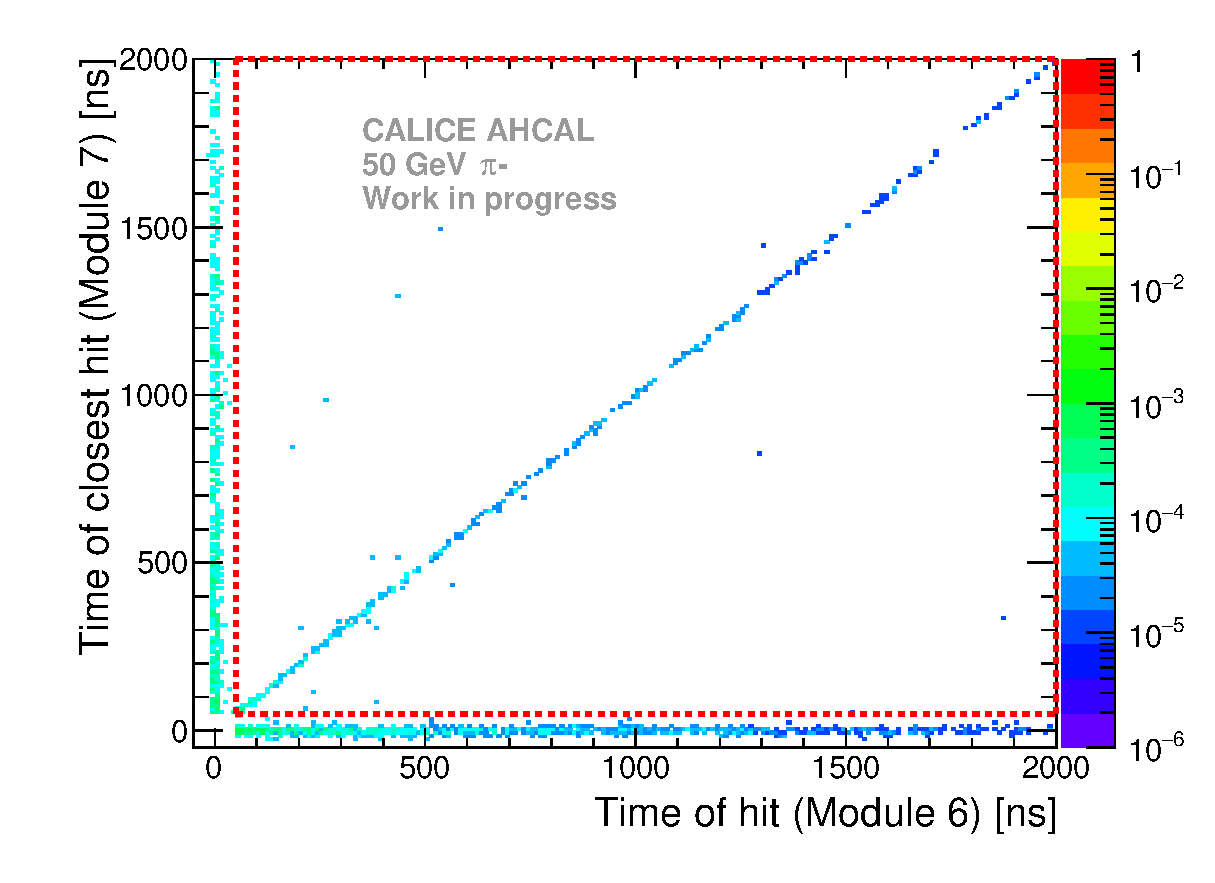
\includegraphics[width=1\textwidth]{../../Draft/fig/Time_Correlation_short.eps}
    \caption{Data} \label{fig:TimeCorr_Data_short_50GeV}
  \end{subfigure}
  \hfill
  \begin{subfigure}[t]{0.49\textwidth}
    \centering
    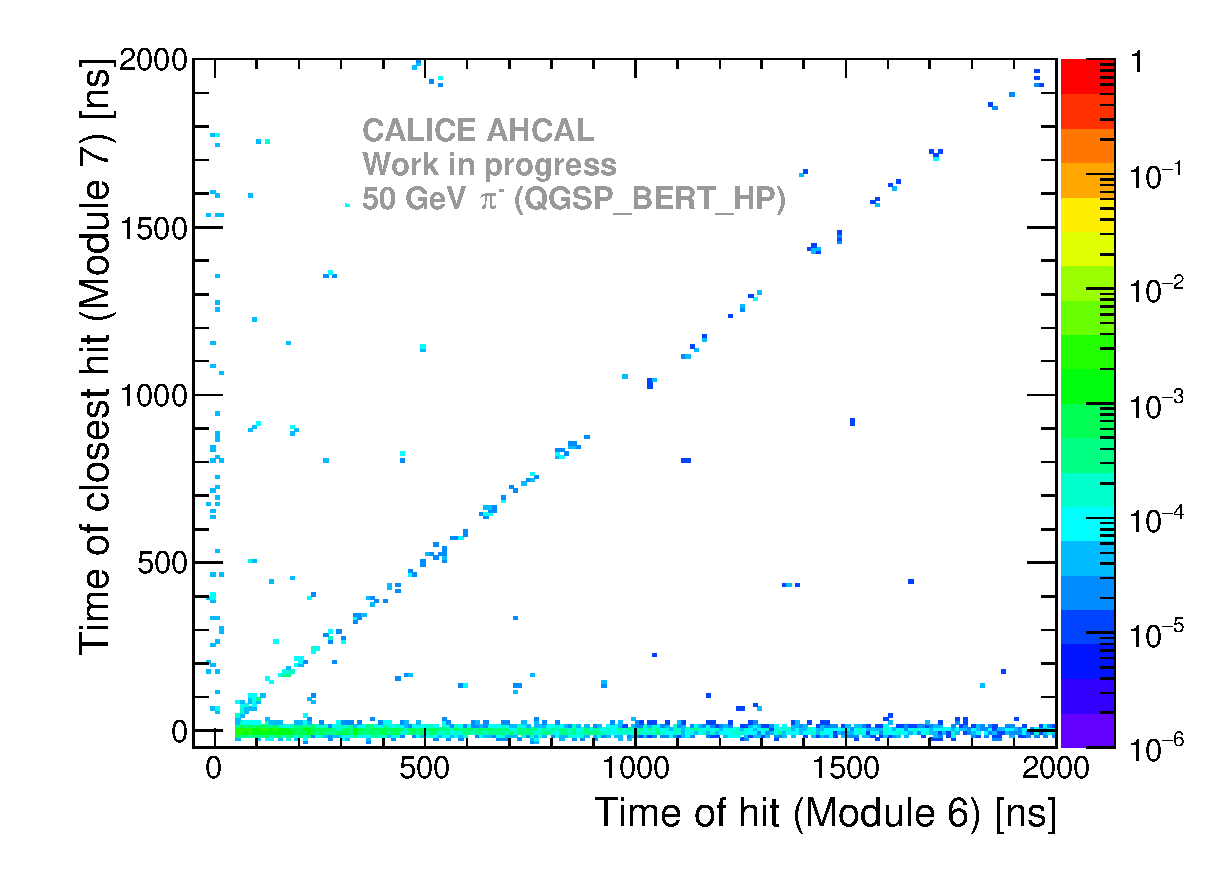
\includegraphics[width=1\textwidth]{../../Draft/fig/Time_Correlation_50GeV_short_QGSPBERTHP_DD4hep.eps}
    \caption{Simulation} \label{fig:TimeCorr_Data_short_50GeV_Sim}
  \end{subfigure}
  \caption{Hit timing correlations between modules 6 and 7 for data on the left and the \ddhep simulation with QGSP\_BERT\_HP on the right, for 50 GeV pions. Each bin is normalized to the total number of entries in the 2D histogram. The red box in the left plot represents the zone investigated to quantify the difference between data and simulation as stated in the text.}
  \label{fig:TimeCorr_short_50GeV}
\end{figure}

\begin{figure}[htbp!]
  \begin{subfigure}[t]{0.49\textwidth}
    \centering
    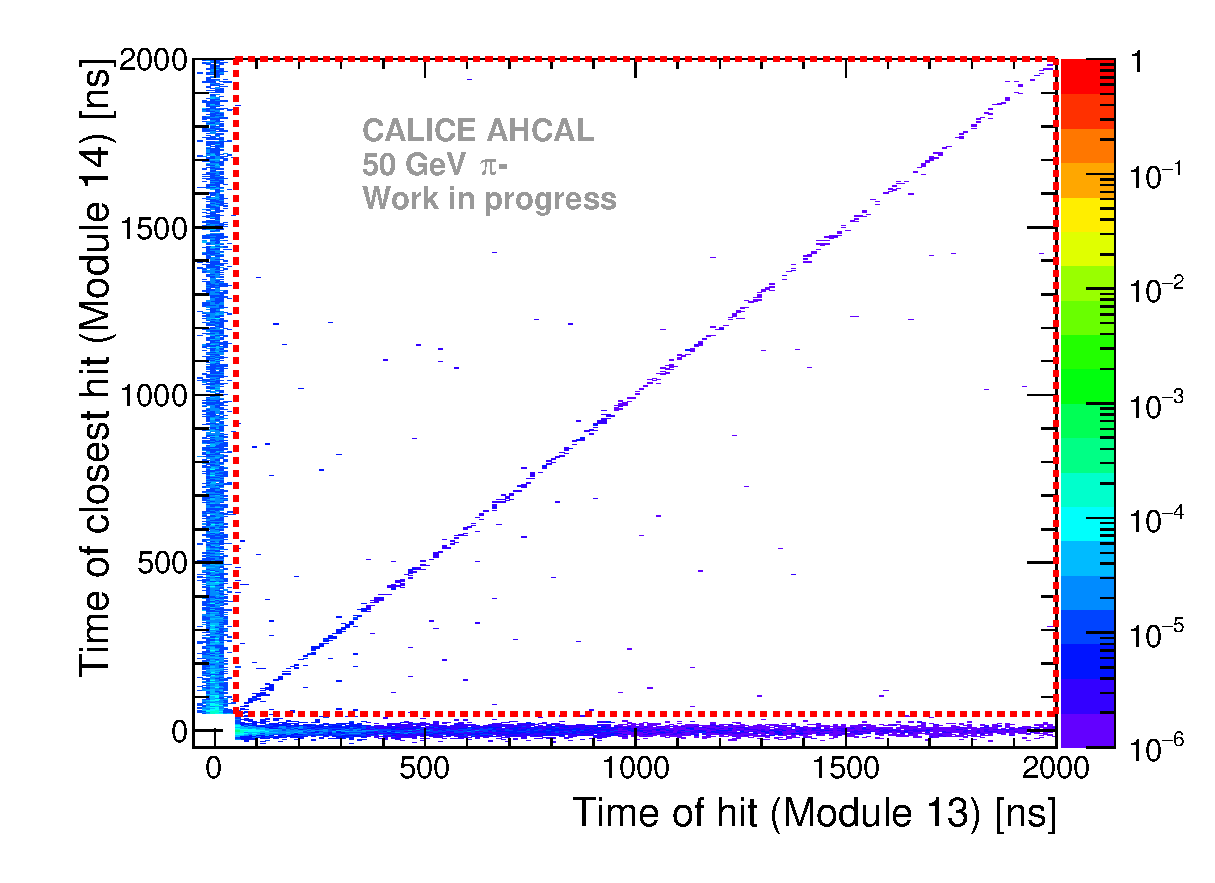
\includegraphics[width=1\textwidth]{../../Draft/fig/Time_Correlation_long.eps}
    \caption{Data} \label{fig:TimeCorr_Data_long_50GeV}
  \end{subfigure}
  \hfill
  \begin{subfigure}[t]{0.49\textwidth}
    \centering
    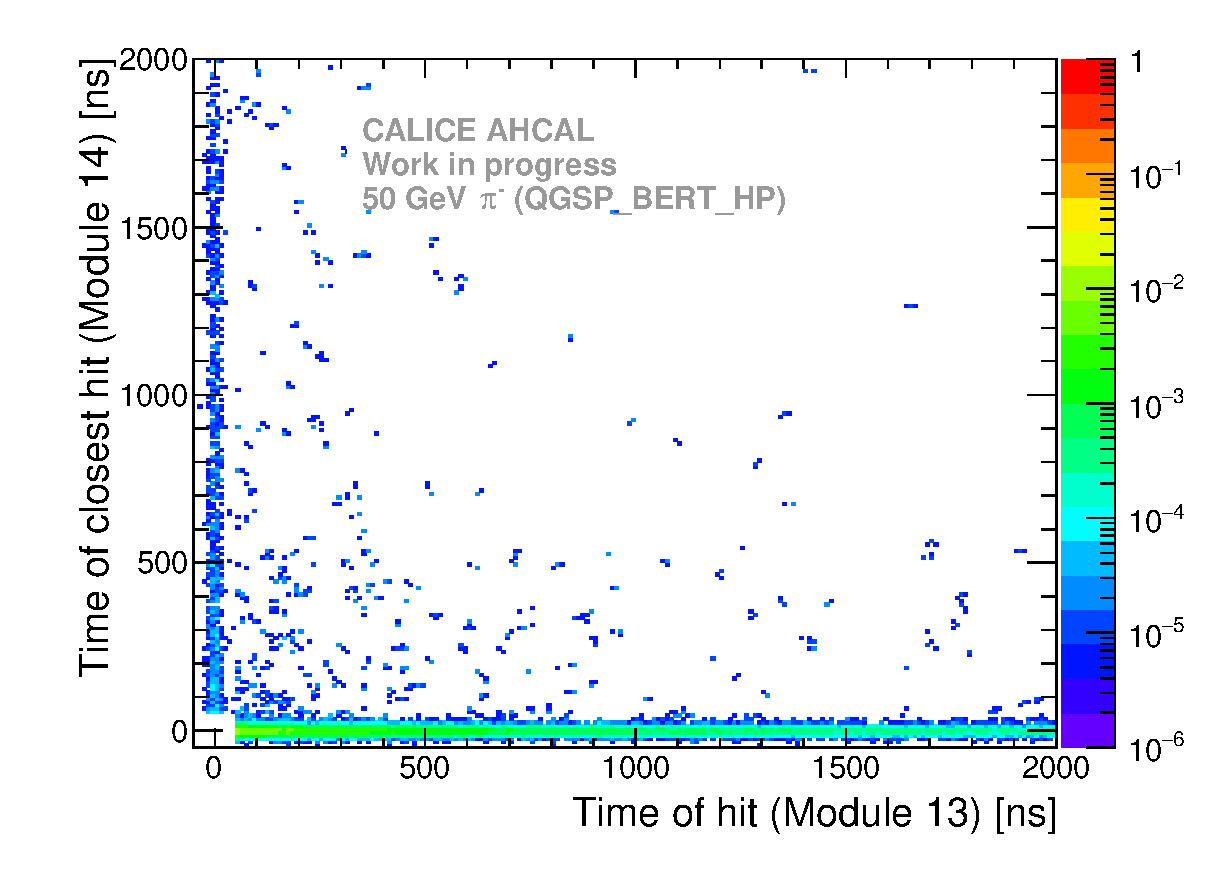
\includegraphics[width=1\textwidth]{../../Draft/fig/Time_Correlation_50GeV_long_QGSPBERTHP_DD4hep.eps}
    \caption{Simulation} \label{fig:TimeCorr_Data_long_50GeV_Sim}
  \end{subfigure}
  \caption{Hit timing correlations between modules 13 and 14 for data on the left and the \ddhep simulation with QGSP\_BERT\_HP on the right, for 50 GeV pions. Each bin is normalized to the total number of entries in the 2D histogram. The red box in the left plot represents the zone investigated to quantify the difference between data and simulation as stated in the text.}
  \label{fig:TimeCorr_long_50GeV}
\end{figure}

\begin{figure}[htbp!]
  \begin{subfigure}[t]{0.49\textwidth}
    \centering
    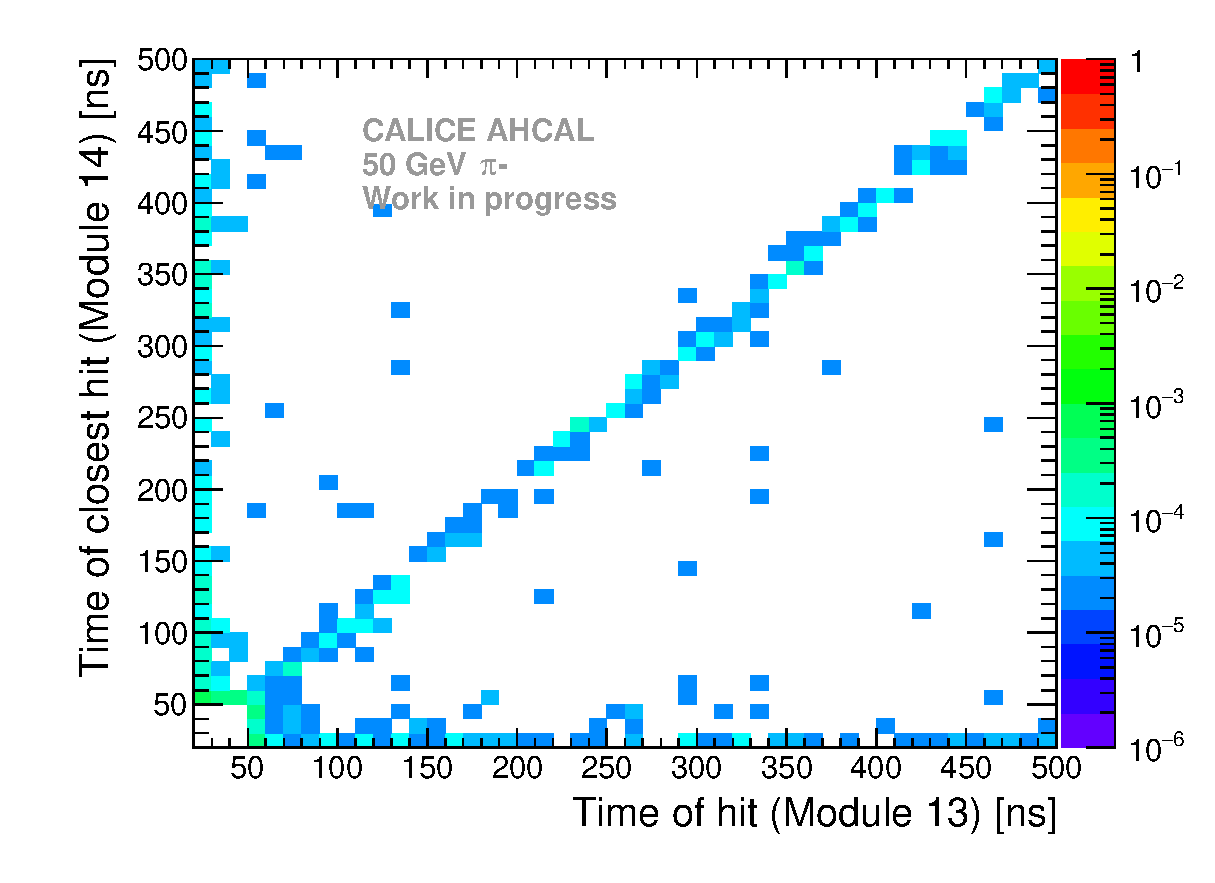
\includegraphics[width=1\textwidth]{../../Draft/fig/Time_Correlation_long_Zoom.eps}
    \caption{Data} \label{fig:TimeCorr_Data_long_50GeV_Zoom}
  \end{subfigure}
  \hfill
  \begin{subfigure}[t]{0.49\textwidth}
    \centering
    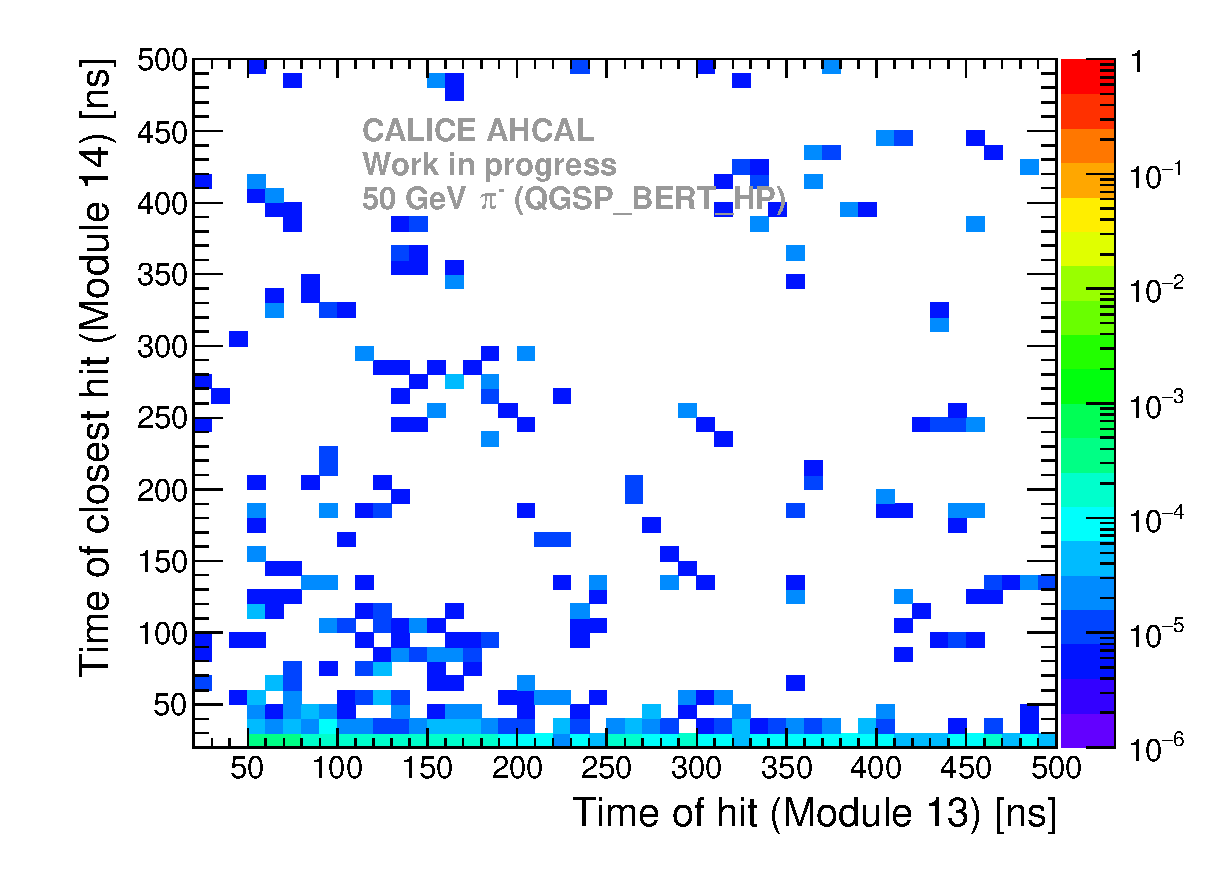
\includegraphics[width=1\textwidth]{../../Draft/fig/Time_Correlation_50GeV_long_QGSPBERTHP_DD4hep_Zoom.eps}
    \caption{Simulation} \label{fig:TimeCorr_Data_long_50GeV_Sim_Zoom}
  \end{subfigure}
  \caption{Hit timing correlations between modules 13 and 14 for data on the left and the \ddhep simulation with QGSP\_BERT\_HP on the right, for 50 GeV pions zoomed in the range [25, 500] ns. Each bin is normalized to the total number of entries in the 2D histogram. The red box in the left plot represents the zone investigated to quantify the difference between data and simulation as stated in the text.}
  \label{fig:TimeCorr_long_50GeV_Zoom}
\end{figure}

\newpage
\section{Additional Plots Second Draft}

\begin{figure}[htbp!]
  \begin{subfigure}[t]{0.49\textwidth}
    \centering
    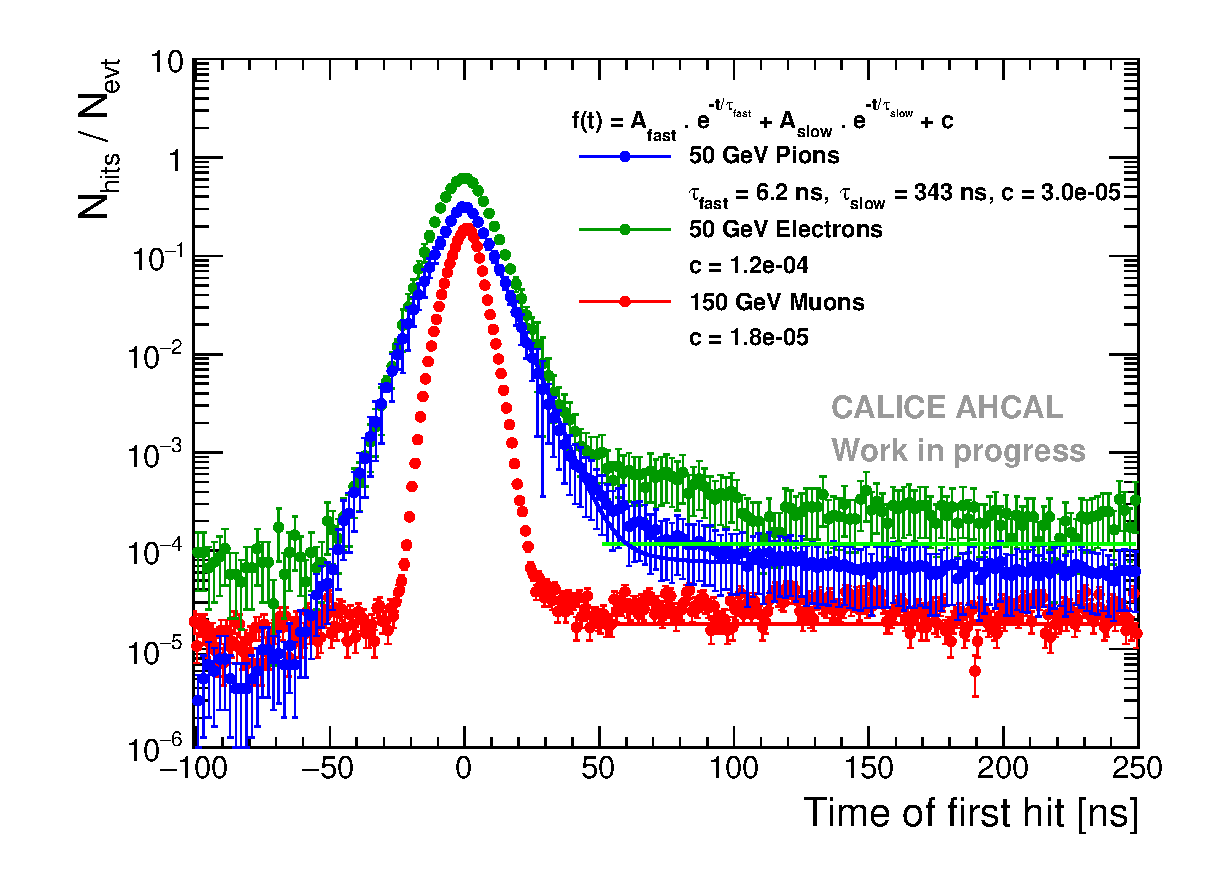
\includegraphics[width=1\textwidth]{../../Draft/fig/Timing_dNdt_Comparison_50GeVe.eps}
    \caption{} \label{fig:dNdt_Data_50GeVe}
  \end{subfigure}
  \hfill
  \begin{subfigure}[t]{0.49\textwidth}
    \centering
    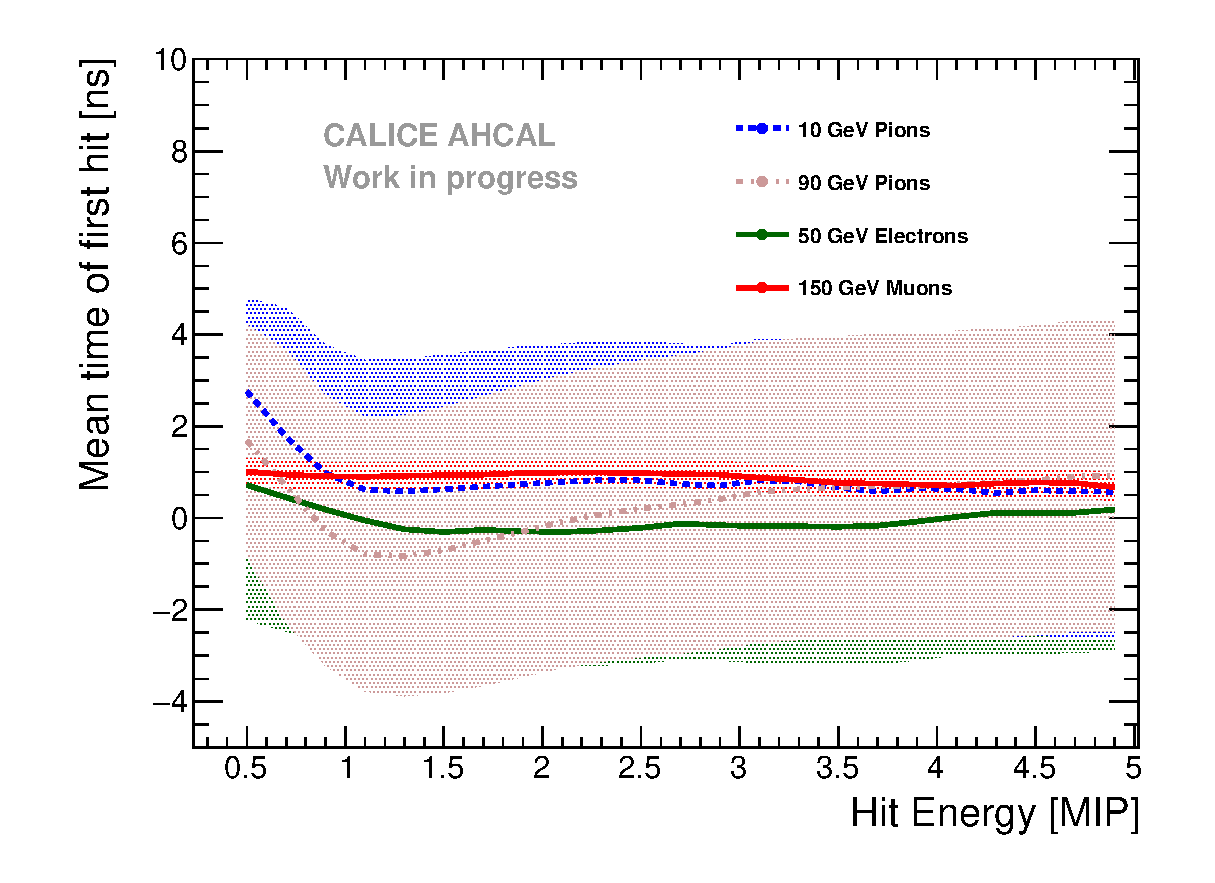
\includegraphics[width=1\textwidth]{../../Draft/fig/Timing_Energy_Comparison_ShortAsymRange.eps}
    \caption{} \label{fig:Energy_Data_all}
  \end{subfigure}
  \caption{On the left, Time of first hit for muons, electrons and pions in steel absorber in a range of -100 to 250 ns. The histograms are normalized to the number of events where at least one hit was identified. The errors bars are statistical and systematic uncertainties. On the right, Comparison of the mean time of first hit as a function of the hit energy in data for muons, electrons and pions. The grey band shows the statistical and systematic uncertainties for pions.}
\end{figure}

\begin{table}[htb!]
  \centering
  \caption{Fit results of the double exponential for each pion energies.}
  \label{table:expotime_pions}
  \begin{tabular}{@{} lccc @{}}
    \toprule
    Pion energy [GeV] & $\tau_{fast}$ [ns] & $\tau_{slow}$ [ns] & c \\
    \midrule
    10 & $5.61 \pm 0.36$ & $285 \pm 52$ & 5.9e-6 \\
    \midrule
    30 & $6.05 \pm 0.32$ & $310 \pm 41$ & 1.4e-5 \\
    \midrule
    50 & $6.21 \pm 0.30$ & $343 \pm 39$ & 3.0e-5 \\
    \midrule
    70 & $7.19 \pm 0.31$ & $333 \pm 35$ & 5.4e-5 \\
    \midrule
    90 & $7.41 \pm 0.32$ & $320 \pm 33$ & 3.0e-5 \\
    \bottomrule
  \end{tabular}
\end{table}

\end{document}
